\subsubsection{MIInsightsPanel Component}
Το MIInsightsPanel Component είναι το τέταρτο και τελευταίο Component που βρίσκεται μέσα στο MIDashboard Component.
Περιέχει πολλά Component ίδιου τύπου MICard Component. Το κάθε MICard Component είναι μια "κάρτα" που εμφανίζει ένα στοιχείο για ένα άτομο, μια ταινία, μια εταιρία παραγωγής, μια χώρα παραγωγής η ένα είδος ταινίας. Για παράδειγμα αν μια κάρτα για μια ταινία με τα μεγαλύτερα έσοδα θα εμφανιζόταν όπως στο σχήμα \ref{layout:micard_revenue}.

\begin{figure}[h]
  \centering
  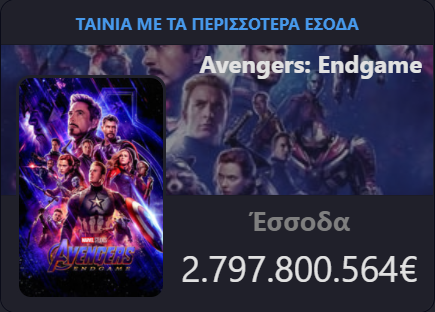
\includegraphics[width=50mm]{Chapters/5 - Architecture/Client/Images/micard_revenue.png}
  \caption{MICard Component}
  \label{layout:micard_revenue}
\end{figure}

Το MICard Component είναι ένα Component το οποιο έχει σχεδιαστεί με ρευστή διάταξη και δυναμικό περιεχόμενο. Ανάλογα με το τι περιεχόμενο θα του δοθεί θα αλλάξει την διάταξη του και θα εμφανίσει τα ανάλογα δεδομένα. Υποστηρίζει Placeholders για την αναμονή των απομακρυσμένων δεδομένων εμφανίζοντας ένα Spinner, και υποστηρίζει και την εμφάνιση ενός μηνύματος λάθους σε περίπτωση που τα δεδομένα για την συγκεκριμένη κατηγορία δεν υπάρχουν. Επιπρόσθετα κάθε Component τυπου MICard μπορεί να πατηθεί σαν κουμπί και ανάλογα με το περιεχόμενο αλλάζει την διεύθυνση στην γραμμή διεύθυνσης του Browser, έτσι ώστε να εμφανιστούν τα ανάλογα δεδομένα μετέπειτα απο το Dashboard Module. Όλα τα MICard λειτουργούν με τον ίδιο τρόπο εκτός απο το MICard που περιέχει δεδομένα ταινιών. Καθώς ο ρόλος της εφαρμογής δεν είναι να εμφανίζει αναλυτικά στοιχεία για ταινίες επειδή υπάρχουν ήδη πολυ γνωστές υπηρεσίες για αυτόν τον σκοπό όπως προαναφέρθηκαν το IMDb και το TMDb, όταν πατηθεί ένα MICard με περιεχόμενο ταινιών θα εμφανιστεί ενα παράθυρο πάνω απο την εφαρμογή το οποίο είναι το MIMovieInfoModal Component όπως φαίνεται στον κώδικα \ref{code:micard_click}.
\begin{figure}[H]
    \begin{TypeScriptcode}
|\textbf{renderCardLinked}|() {
  const link = this.state.entity?AppUtils.|\textbf{generateNavigationLink}|(this.state.entity):''
  return (<NavLink className="mi-card-link" onClick={this.onLinkClick} to={link}>{this.renderCard()}|</NavLink>|);
}
_render() {
  return (
    <>
      {this.state.loaded && this.state.entity ?this.|\textbf{renderCardLinked}|() : this.renderCard()}
      {this.props.entityType === TmdbEntityType.MOVIE ?(|\textbf{<MIMovieInfoModal}| open={this.state.modal} onClose={() => this.setState({modal: false})} entity={this.props.entity as any}|\textbf{/>}|) : null}
    |</>|
  )
}
    \end{TypeScriptcode}
    \caption{Αλγόριθμος αλλαγής διεύθυνσης από το MIRolePicker Component.}
   \label{code:micard_click}
\end{figure}


Το MIMovieInfoModal Component περιέχει το πόστερ της ταινίας καθώς και μια εικόνα background σχετική με την ταινία και περιέχει τα πολύ βασικά στοιχεία που χρησιμοποιεί η εφαρμογή όπως, τα έσοδα, τα έξοδα, την βαθμολογία με της ψήφους της ταινίας καθώς και το πόσο διαρκεί η ταινία συνολικά. Επιπρόσθετα δίνει την επιλογή για περισσότερα στοιχεία για αυτήν την ταινία προσφέροντας 2 συνδέσμους ανακατεύθυνσης που ο ένας πηγαίνει τον χρήστη στον ισότοπο του TMDb στην επιλεγμένη ταινία και ο άλλος στο IMDB όπως φαίνεται στο σχήμα \ref{layout:mimoviemodal}

\begin{figure}[H]
  \centering
  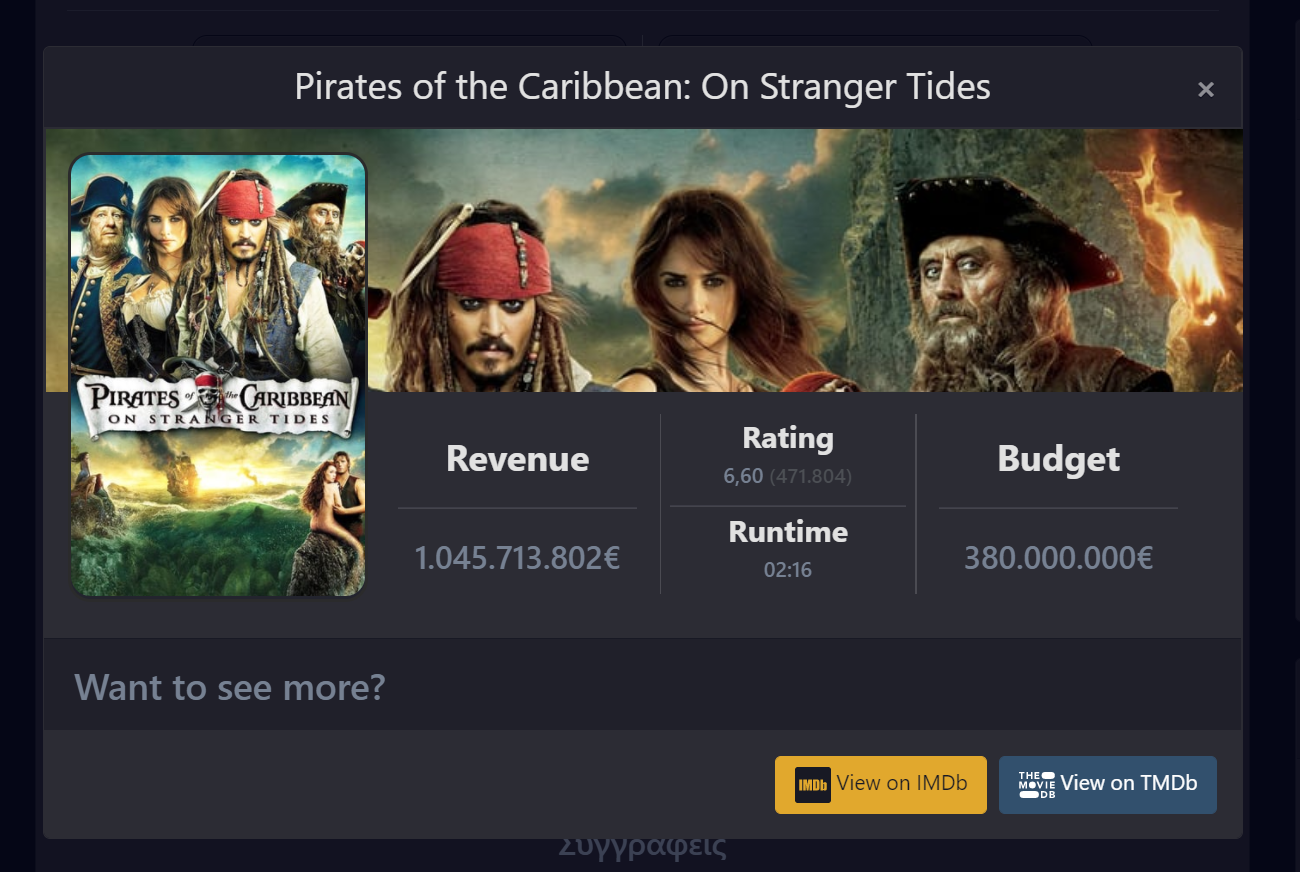
\includegraphics[width=100mm]{Chapters/5 - Architecture/Client/Images/mimoviemodal.png}
  \caption{MIMovieInfoModal Component}
  \label{layout:mimoviemodal}
\end{figure}